\documentclass[tikz,border=10pt]{standalone}
\usepackage{tikz-feynman}

\begin{document}
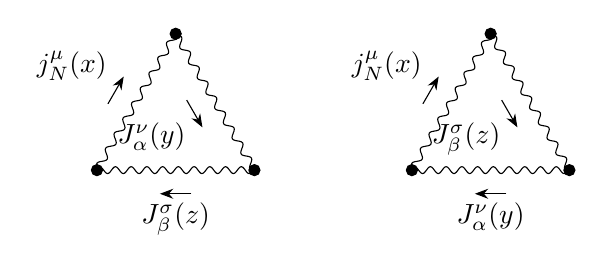
\begin{tikzpicture}
  \begin{feynman}
    \vertex (a) at (0,0);
    \vertex (b) at (2,0);
    \vertex (c) at (1,1.732); % 120 degree separation for equilateral triangle
    \vertex (d) at (1,0.577); % Center point for the arrows
    
    % First triangle
    \diagram* {
      (a) -- [photon, momentum={[arrow shorten=0.4]\(j_N^\mu(x)\)}] (c),
      (c) -- [photon, momentum'={[arrow shorten=0.4]\(J_\alpha^\nu(y)\)}] (b),
      (b) -- [photon, momentum={[arrow shorten=0.4]\(J_\beta^\sigma(z)\)}] (a)
    };
    
    % Adding arrows in the middle of the lines for chiral nature
    \draw [fill=black] (a) circle (2pt);
    \draw [fill=black] (b) circle (2pt);
    \draw [fill=black] (c) circle (2pt);
    
    % Second triangle, mirrored
    \vertex (a2) at (4,0);
    \vertex (b2) at (6,0);
    \vertex (c2) at (5,1.732);
    \vertex (d2) at (5,0.577);
    
    \diagram* {
      (a2) -- [photon, momentum={[arrow shorten=0.4]\(j_N^\mu(x)\)}] (c2),
      (c2) -- [photon, momentum'={[arrow shorten=0.4]\(J_\beta^\sigma(z)\)}] (b2),
      (b2) -- [photon, momentum={[arrow shorten=0.4]\(J_\alpha^\nu(y)\)}] (a2)
    };
    
    \draw [fill=black] (a2) circle (2pt);
    \draw [fill=black] (b2) circle (2pt);
    \draw [fill=black] (c2) circle (2pt);
    
  \end{feynman}
\end{tikzpicture}
\end{document}